\begin{abstract}

This project tests whether independently trained recurrent agents can
learn useful message meanings in a task with complementary private
information. A scout knows the target and a runner must collect it, with
the target hidden from the runner and a wall blocking physical
interaction. I adapt independent PPO with a cue-directed
positive-signalling objective, without assigning symbols to targets or
adding a listener-specific loss. Across 20 seeds per condition, discrete
communication reaches 87.6\% (95\% CI 86.3--88.6) held-out success, with
a +65.0 pp (95\% CI +63.5 to +66.3) advantage over no communication. A
message-permutation intervention removes +67.6 pp (95\% CI +66.0 to
+69.1), distinguishing informative speech from actual listener use. A
separately pre-registered extension introduces two-word messages and
color--shape targets. It supports communication on seen combinations but
fails the frozen generalization criterion. A continuous vocal channel
provides an exploratory comparison. The contribution is a controlled,
reproducible test of a task-specific signalling modification and the
limits of the resulting protocols, rather than a claim that symbolic
communication or positive signalling is new.

\end{abstract}

\section{Question}\label{question}

Can two independently learning agents develop and use a communication
protocol that improves coordinated action when message meanings are
never programmed? Two recurrent reinforcement-learning agents share a
task that neither can reliably solve from its own observations. They can
exchange one symbol from an 8-symbol vocabulary per step, and the
symbols start out meaningless. I test whether a protocol emerges,
whether it improves joint success on unseen maps, and whether the
agents' behavior \emph{causally} depends on it. A minimal, controlled
environment makes the last question answerable; this is not a model of
language.

\subsection{Contribution and connection to the
course}\label{contribution-and-connection-to-the-course}

The starting method is independent recurrent PPO (Schulman et al., 2017;
de Witt et al., 2020). The specific modification is an auxiliary
objective that makes the scout's messages informative about its private
target cue. The task contribution is to direct the signalling pressure
toward the missing information needed by the partner, while leaving the
symbol assignment and listener policy learned. The direct ablation
removes only this objective. Channel controls answer a different
question: whether a trained communicating pair benefits from receiving
informative messages. Keeping these comparisons separate prevents a
communication advantage from being mistaken for evidence about which
training component caused it.

This connects directly to \textbf{Topic 7: AI Agents}, particularly the
course's agent reinforcement learning and multi-agent systems material.
A policy maps local state to actions, a GRU supplies short-term memory,
and shared task feedback trains coordination between separate agents.
Unlike the course's language-model agent examples, these agents have no
pretrained language, tool descriptions, planner prompts, or externally
supplied dictionary. Their knowledge is encoded in the policies, and the
channel is a learned interface between their different observations. The
experiment therefore isolates a small part of the broader
knowledge-system problem: getting information held by one component to
influence another component's decisions.

\subsection{Relation to prior work}\label{relation-to-prior-work}

Foerster et al.~(2016) study learned communication in multi-agent
reinforcement learning, and Lazaridou et al.~(2017) study coordination
through emergent symbols. This project follows that research direction
in an intentionally small navigation task. It does not claim to
introduce emergent communication or to outperform those systems on their
benchmarks.

The closest methodological antecedent is Eccles et al.~(2019), who
introduce positive-signalling and positive-listening biases. Their
signalling objective relates messages to a speaker's trajectory. Here
the statistic groups message distributions by the private target cue, a
task-specific adaptation that ignores nuisance variation in the scout's
position. I retain ordinary reward-based listener learning. Comparing
against unbiased IPPO isolates the added cue-directed term; it does
\textbf{not} establish that this adaptation outperforms Eccles et al.'s
original full method. An equal-budget implementation of their trajectory
objective would be needed for that stronger claim.

Lowe et al.~(2019) show why message correlations can be misleading when
listeners do not use the channel. This motivates the interventions and
the explicit comparison with informative but unheard scouts. Chaabouni
et al.~(2020) distinguish structural compositionality from
generalization to new combinations. The second experiment follows that
distinction: task transfer, property-level structure and intervention
sensitivity are measured separately, and none alone licenses a
language-like compositionality claim.

\section{Environment and information
structure}\label{environment-and-information-structure}

The world is a deterministic, seeded 12×12 grid split by a solid wall.

\begin{itemize}
\tightlist
\item
  \textbf{The scout} sits in a control room. It is the only agent told
  which of four item types (A--D) is wanted, but it can never reach an
  item.
\item
  \textbf{The runner} sits in the warehouse with all four items, the
  depot, and 8 obstacles. It sees a 7×7 egocentric window but never sees
  the target.
\item
  \textbf{Dynamics:} each step, each agent moves (or interacts) and
  emits a symbol, which the partner hears one step later. Picking up an
  item earns +0.1 and each step costs −0.01. Delivering the target earns
  +1 and ends the episode. Delivering a wrong item also ends it, as a
  failure, so guessing succeeds at most 1/4 of the time.
\item
  \textbf{Episode sampling:} an episode is accepted only if \emph{every}
  item is deliverable in time, and the target is drawn afterwards. This
  keeps the geometry from revealing the target.
\item
  \textbf{Information path:} other-agent positions are absent from
  observations, and the uncued runner's target block is zero. The scout
  cannot reach items. Messages provide the target-information path in
  this base task.
\item
  \textbf{Layouts:} 48 are used for training; 24 held-out layouts are
  used only for evaluation.
\end{itemize}

Perception is a square crop rather than line-of-sight vision. A v1 or
vocal scout near the wall can see warehouse cells across it; the wall
blocks movement. V2 explicitly masks the scout's warehouse content. This
distinction does not reveal the private cue or scout position to the
uncued runner, but limits claims about visual separation.

A scripted team with privileged map knowledge confirms that the task can
be solved reliably with communication, while the no-message reference
remains near guessing. On held-out layouts it succeeds 100.0\% of the
time with a fixed codebook and 100.0\% with the runner told the target.
With no communication it succeeds 26.5\% of the time, and with random
symbols 25.0\%.

\begin{figure}[tb]
\centering
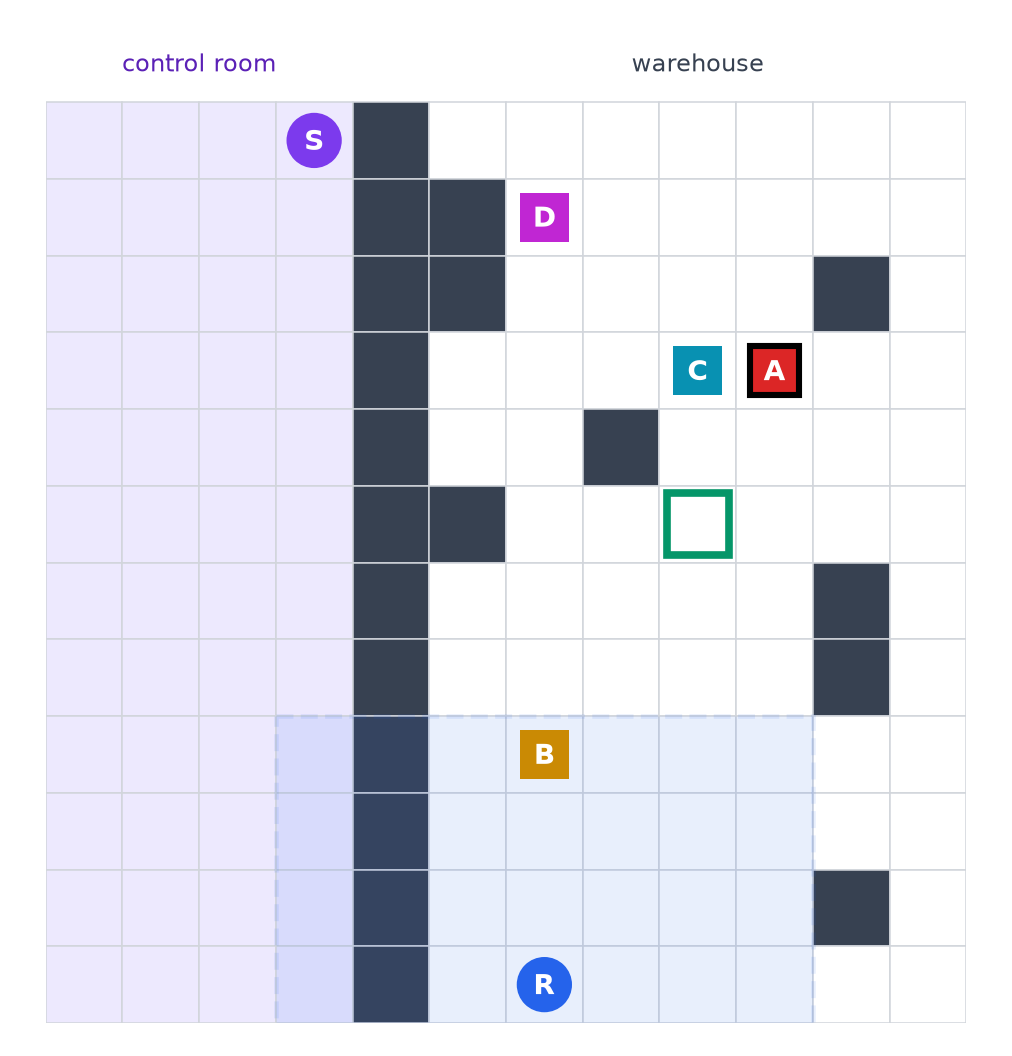
\includegraphics[width=\linewidth]{images/map.png}
\caption{The partition separates private target knowledge from the warehouse. This schematic explains the observation design; it is not an evaluation outcome.}
\end{figure}

\section{Conditions and controls}\label{conditions-and-controls}

All four learned conditions share the observation space (315 features),
the action space (6 moves × 8 symbols), the architecture, the
hyperparameters, and the training budget. The three partial-information
controls differ in delivered message content; the oracle additionally
reveals the target to the runner:

\begin{center}
\small
\resizebox{\columnwidth}{!}{%
\begin{tabular}{@{}lll@{}}
\toprule\noalign{}
Condition & Runner sees target & What the runner hears \\
\midrule\noalign{}



Learned comm & no & the scout's last symbol \\
No comm & no & always ``silence'' \\
Random messages & no & a uniformly random symbol \\
Oracle (reference) & yes & always ``silence'' \\

\bottomrule
\end{tabular}}
\end{center}

The random-message control separates \emph{information} from mere extra
input variability. The oracle provides a learned navigation reference
with target knowledge. At evaluation time the comm runs are also tested
with their symbols \textbf{permuted}: each episode applies its own
random relabeling of the 8 symbols. They are also tested
\textbf{silenced}. If the runner relies on what particular symbols mean,
both interventions should push success toward chance.

\section{Method}\label{method}

Each agent is its own actor-critic network (independent PPO):

\begin{itemize}
\tightlist
\item
  Architecture: a two-layer MLP, then a GRU with 128 units, then heads
  for the move, the symbol, and the value.
\item
  No shared parameters and no centralized critic.
\item
  The move and the symbol are sampled jointly and trained with the same
  PPO objective.
\item
  Training ran on 64 parallel environments, with 128-step rollouts and
  learning rate 1e-3, for 10.0 M environment steps per run. Every agent
  in every condition also received a cue-informativeness bias with
  weight 0.2, a targeted form of the positive-signalling bias of Eccles
  et al.~(2019): it rewards symbols that depend on the agent's private
  target cue, and never specifies which symbol should mean what.
\end{itemize}

\subsection{The single changed
component}\label{the-single-changed-component}

For cued samples in a minibatch, let \(q_i(m)\) be the agent's predicted
message distribution, \(c_i\) its private cue, \(\bar q_c(m)\) the mean
distribution for cue \(c\), and \(\bar q(m)\) the overall mean. The
objective estimates cue information as

\[\widehat I(M;C)=H(\bar q)-\sum_c \widehat p(c)H(\bar q_c).\]

The added loss is \(-\lambda\widehat I(M;C)\), with the frozen
coefficient \(\lambda=0.2\). Entropies in the training objective use
natural logarithms; the reported descriptive MI uses bits. An agent with
no visible cue contributes zero. This rewards different distributions
across cues without choosing the symbol associated with any cue. In
particular, the objective receives private cue categories but no
correct-message labels. It is a deliberate inductive bias, so the result
should not be described as communication emerging without any structural
guidance.

Ordinary PPO uses clipped policy updates, a local value loss,
generalized advantage estimation and entropy bonuses. Movement and
message log probabilities are summed for the joint action. Recurrent
training uses truncated backpropagation through the rollout, resetting
state at episode boundaries. Both agents have separate parameters and
optimizers. The listener receives no gradient through the channel and no
supervised decoder target.

\begin{center}
\small
\resizebox{\columnwidth}{!}{%
\begin{tabular}{@{}ll@{}}
\toprule\noalign{}
Frozen optimization setting & Value \\
\midrule\noalign{}



Discount / GAE coefficient & 0.99 / 0.95 \\
PPO clipping / gradient clipping & 0.2 / 0.5 \\
Epochs / environment minibatches & 4 / 4 \\
Value-loss coefficient & 0.5 \\
Move / message entropy coefficients & 0.01 / 0.01 \\

\bottomrule
\end{tabular}}
\end{center}

Each condition was trained with 20 independent seeds, for 80 runs in
total. Evaluation:

\begin{itemize}
\tightlist
\item
  Every run was evaluated on the same 200 held-out-layout episodes, with
  stochastic policies and a fixed evaluation seed.
\item
  Every run was also evaluated on 200 training-layout episodes, which
  gives the generalization gap.
\item
  95\% confidence intervals use a percentile bootstrap over seeds
  (10,000 resamples). Between-condition differences resample the two
  conditions independently. Interventions and gaps are paired within a
  run.
\end{itemize}

The hypotheses were pre-registered before any benchmark seed was
trained:

\begin{itemize}
\tightlist
\item
  \textbf{H1:} the comm − no-comm gain is at least 15 pp, with a CI that
  excludes 0.
\item
  \textbf{H2:} the intact − permuted drop is at least 10 pp, with a CI
  that excludes 0.
\end{itemize}

The independent unit is a trained seed, not an evaluation episode. The
repeated episodes estimate a particular policy's performance; the seed
bootstrap represents training variability. The fixed episode set
improves comparability but does not represent uncertainty across
arbitrary map generators. Evaluation is stochastic under the same fixed
generator seed, and every reported checkpoint is the final one. Held-out
outcomes never select a checkpoint, pilot setting or training budget.

\section{Results}\label{results}

\begin{center}
\small
\resizebox{\columnwidth}{!}{%
\begin{tabular}{@{}
  >{\raggedright\arraybackslash}p{(\linewidth - 6\tabcolsep) * \real{0.2500}}
  >{\raggedright\arraybackslash}p{(\linewidth - 6\tabcolsep) * \real{0.2500}}
  >{\raggedright\arraybackslash}p{(\linewidth - 6\tabcolsep) * \real{0.2500}}
  >{\raggedright\arraybackslash}p{(\linewidth - 6\tabcolsep) * \real{0.2500}}@{}}
\toprule\noalign{}
\begin{minipage}[b]{\linewidth}\raggedright
Condition
\end{minipage} & \begin{minipage}[b]{\linewidth}\raggedright
Held-out success
\end{minipage} & \begin{minipage}[b]{\linewidth}\raggedright
Train-layout success
\end{minipage} & \begin{minipage}[b]{\linewidth}\raggedright
Steps / success
\end{minipage} \\
\midrule\noalign{}



Learned comm & 87.6\% (95\% CI 86.3--88.6) & 83.7\% (95\% CI 82.6--84.8)
& 16.9 \\
No comm & 22.5\% (95\% CI 21.8--23.3) & 21.0\% (95\% CI 20.3--21.7) &
15.5 \\
Random messages & 22.3\% (95\% CI 21.5--23.2) & 21.2\% (95\% CI
20.4--22.1) & 15.3 \\
Oracle & 93.1\% (95\% CI 92.4--93.8) & 90.6\% (95\% CI 89.8--91.3) &
15.9 \\

\bottomrule
\end{tabular}}
\end{center}

\begin{figure}[tb]
\centering
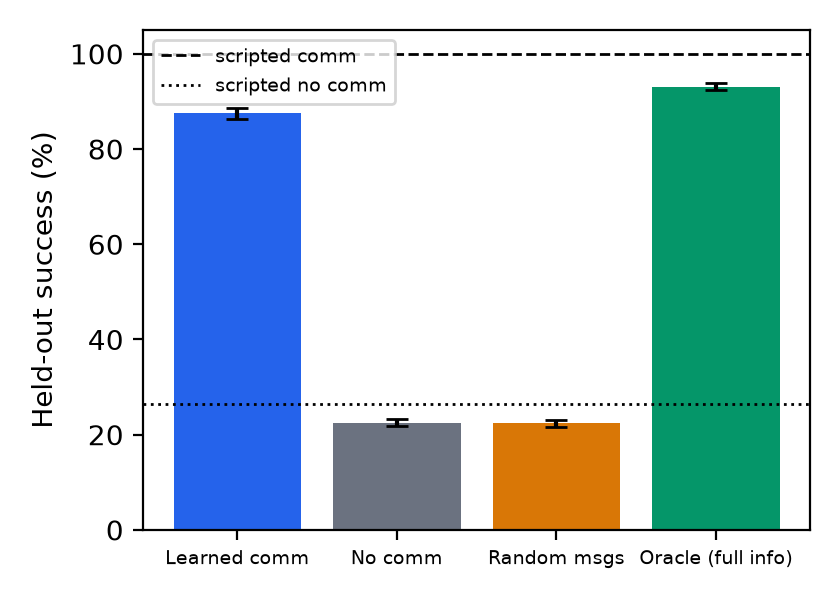
\includegraphics[width=\linewidth]{images/fig_success.png}
\caption{Held-out success (mean over 20 seeds, 95\% bootstrap CI). Dashed and dotted lines: scripted comm and no-comm references.}
\end{figure}

\begin{itemize}
\tightlist
\item
  \textbf{H1 (gain):} comm − no comm = +65.0 pp (95\% CI +63.5 to
  +66.3).
\item
  \textbf{H2 (causal):} intact − permuted = +67.6 pp (95\% CI +66.0 to
  +69.1); intact − silenced = +74.9 pp (95\% CI +73.0 to +77.0).
\item
  \textbf{Control:} comm − random messages = +65.2 pp (95\% CI +63.7 to
  +66.5).
\item
  \textbf{Generalization gap} (train − held-out) for comm: -3.8 pp (95\%
  CI -5.2 to -2.4). The negative gap also occurs for the oracle (-2.5 pp
  (95\% CI -3.4 to -1.6)), consistent with an easier held-out episode
  set. This fixed comparison does not establish robustness to other map
  distributions or exclude overfitting more generally.
\item
  \textbf{Pre-registered criterion met:} True.
\end{itemize}

\begin{figure}[tb]
\centering
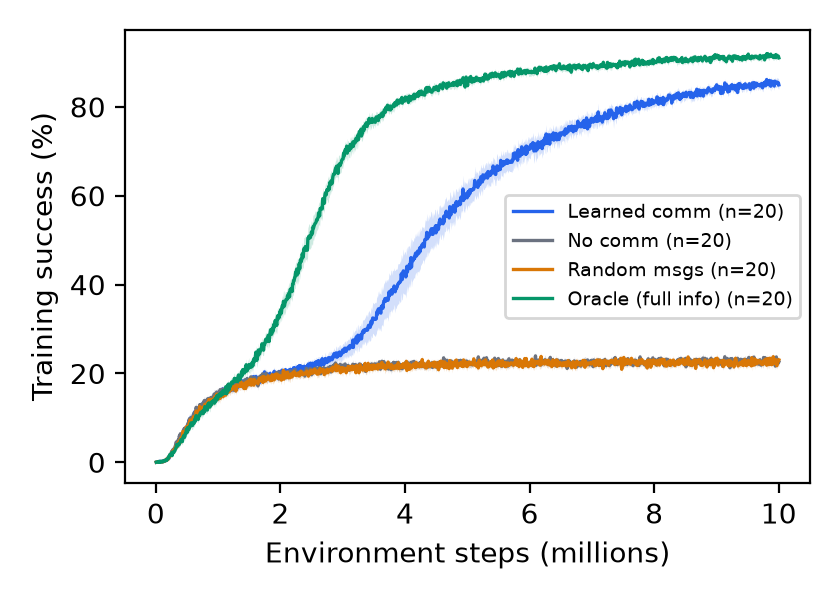
\includegraphics[width=\linewidth]{images/fig_training_curves.png}
\caption{Training-episode success over environment steps (mean $\pm$ 95\% band over seeds).}
\end{figure}

\begin{figure}[tb]
\centering
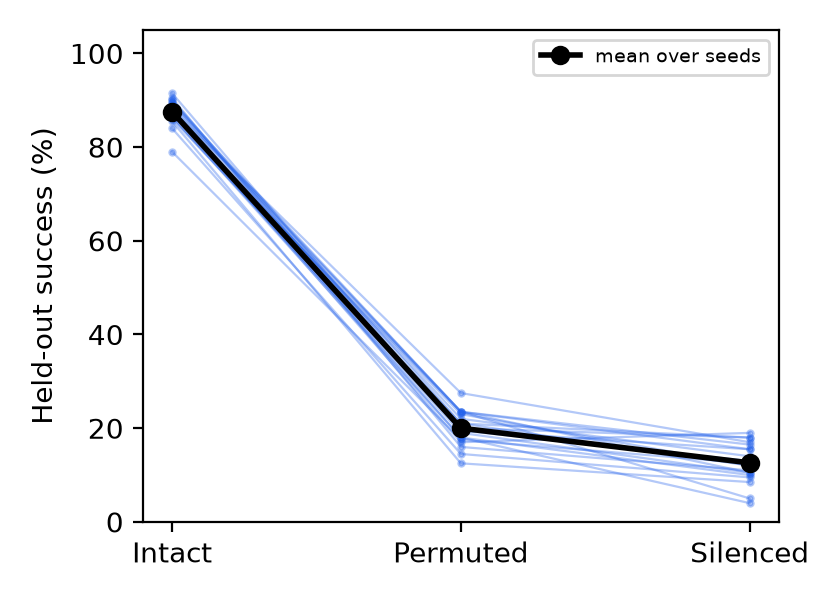
\includegraphics[width=\linewidth]{images/fig_intervention.png}
\caption{Each line is one comm seed evaluated on the same held-out episodes with intact, permuted, and silenced messages.}
\end{figure}

Silencing the channel lowers success even further than permuting it
(+74.9 pp (95\% CI +73.0 to +77.0) vs +67.6 pp (95\% CI +66.0 to
+69.1)), consistent with a runner that always heard a symbol during
training being thrown off by an out-of-distribution ``silence'' input.

\section{What the symbols mean}\label{what-the-symbols-mean}

Mutual information between the target and the scout's first symbol is
1.98 bits for learned comm (the maximum is 2 bits). For comparison, it
is 1.99 bits for no-comm scouts, whose symbols nobody hears, and 1.99
bits for random-message scouts. MI describes the \emph{speaker} only: a
scout can be informative while the runner ignores it. That is why the
permutation test, not MI, carries the causal claim (Lowe et al., 2019).

Because the informativeness bias applies in every condition, scouts
whose symbols are never delivered are just as informative, which is the
clearest demonstration that MI measures the speaker, not the listener.

\begin{figure}[tb]
\centering
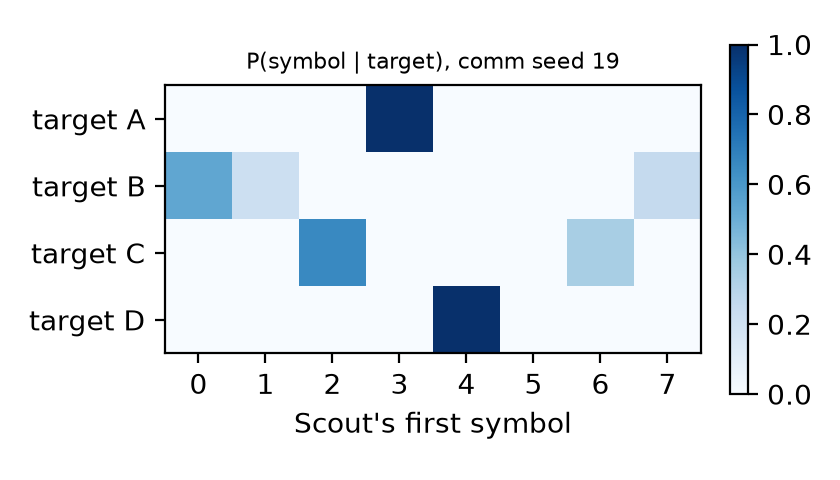
\includegraphics[width=\linewidth]{images/fig_protocol.png}
\caption{P(first symbol \textbar{} target) for the median comm seed.}
\end{figure}

Figure 5 shows that some targets are expressed with more than one symbol
(synonyms), while no symbol is shared between targets.

\section{Discussion}\label{discussion}

The agents invented a working protocol. Learned communication beat the
no-communication control by the margin reported above, on maps they
never trained on. Scrambling the symbol meanings removed the advantage
and reduced performance to roughly guessing levels, so the runner's
behavior depends on what particular symbols mean, not merely on hearing
something. Random messages did not reproduce the gain, supporting the
value of information over input variability alone. Figure 5 shows an
unambiguous code for this representative seed: each used symbol points
to one target, although the assignment differs across seeds. Without the
informativeness bias, the same agents did not develop a protocol within
the three-seed pilot budget (section 11). The bias rewards cue-dependent
messages without specifying their symbol assignment. The listener learns
to use those messages through shared task reward.

\subsection{Original-method
comparison}\label{original-method-comparison}

The original train-only pilots compared three seeds per setting, giving
unbiased comm 21.8\% and biased comm 83.2\%. These were selection
evidence, not a 20-seed test of the method modification. To address that
limitation, a supplementary full-budget comparison was declared on
November 9 after the original outcomes were known. It retains the
architecture, task, PPO settings and benchmark seeds and changes only
the signalling coefficient to zero. It is post-hoc exploratory evidence;
the original pre-registered claims are unchanged.

Across 20 full-budget seeds, unbiased IPPO reaches 22.7\% (95\% CI
21.7--23.6) held-out success, compared with 87.6\% (95\% CI 86.3--88.6)
for cue-directed IPPO. The estimated biased minus unbiased difference is
+64.9 pp (95\% CI +63.3 to +66.4). The unbiased baseline's intact minus
permuted drop is +0.7 pp (95\% CI -0.2 to +1.6). The final-checkpoint
protocol is retained; method differences bootstrap independent seed
sets, while permutation drops pair each policy with itself. The
difference estimate is exploratory because the comparison was added
after the original outcomes were known; it does not retroactively expand
the pre-registered hypotheses.

\subsection{What failures and interventions
establish}\label{what-failures-and-interventions-establish}

An intervention changes the receiver's information while retaining the
learned networks, layouts and target tasks. A drop under a fresh symbol
permutation supports reliance on stable message identities. It does not
show that a message has a human-like semantic interpretation: a learned
joint controller can use arbitrary codes, repeated signals or
history-dependent conventions. Silence is additionally outside the
communicating listener's usual input distribution, so it is a useful
ablation but a less specific test of symbol meaning.

Errors can arise before picking, at target identification, or during
delivery. The oracle is the navigation and control reference, while no
communication and random messages measure performance without a useful
information channel. The representative replay is chosen by the fixed
median-seed rule and illustrates particular successes and failures; it
is not an independent statistical sample or a substitute for aggregate
performance. The v2 property and wrong-pick measures below help
distinguish partial target identification from joint success, but
exclude episodes without a pick where their definitions condition on
picking. Such conditional diagnostics must not be read as overall task
accuracy.

\section{Exploratory extension: a vocal
channel}\label{exploratory-extension-a-vocal-channel}

This arm was declared before pre-registration but is exploratory: it
does not bear on H1 or H2.

\textbf{Setup.}

\begin{itemize}
\tightlist
\item
  Instead of a symbol, each agent emits a continuous ``pitch'' in {[}−1,
  1{]} and hears the other's pitch one step later with Gaussian noise (σ
  = 0.1).
\item
  Task dynamics are retained. A Gaussian pairwise-distance information
  surrogate, inspired by Kolchinsky and Tracey (2017), replaces the
  discrete bias. Because the actual pitches are clipped, it is not
  claimed as an exact bound for the heard channel.
\item
  20 seeds each of vocal comm and vocal no comm were trained and
  evaluated on the same held-out episodes.
\item
  The vocal budget is 20.0 M steps per run, longer than v1; absolute
  rates across arms therefore do not isolate channel type.
\item
  \textbf{The causal test is shuffling:} the runner hears the pitch the
  scout produced in a \emph{different} episode. That keeps the sounds
  realistic but breaks their link to this episode's target.
\end{itemize}

\textbf{Results.}

\begin{itemize}
\tightlist
\item
  \textbf{Held-out success:} vocal comm 73.0\% (95\% CI 69.9--75.8)
  vs.~vocal no comm 21.4\% (95\% CI 20.4--22.6); the gain is +51.5 pp
  (95\% CI +48.3 to +54.6).
\item
  \textbf{Causal:} intact − shuffled = +57.9 pp (95\% CI +54.5 to
  +61.0); intact − silenced = +60.0 pp (95\% CI +56.4 to +63.6).
\item
  \textbf{Binned MI} (target; first pitch, 8 bins): 1.99 bits.
\end{itemize}

\begin{figure}[tb]
\centering
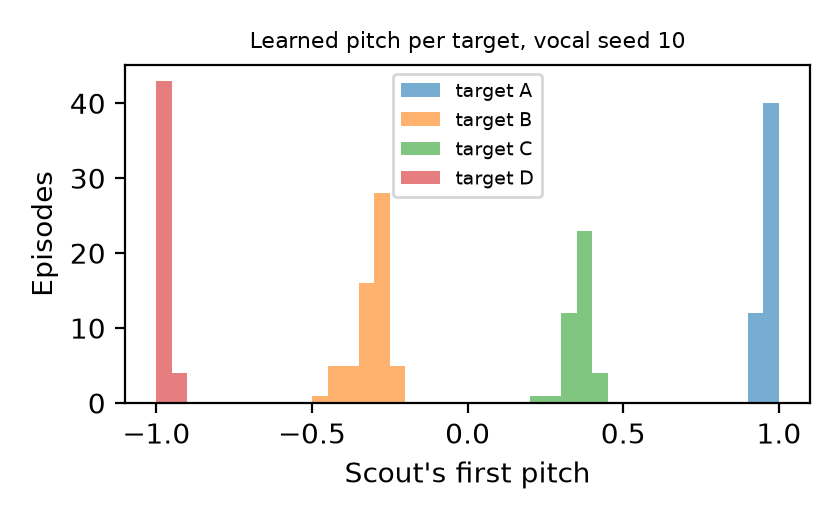
\includegraphics[width=\linewidth]{images/fig_pitch.png}
\caption{The scout's first pitch in each held-out episode, by target, for the median vocal seed. Separate peaks mean the agents invented distinct "notes".}
\end{figure}

Figure 6 shows four sharply separated notes, roughly evenly spaced
across the pitch range: the agents carved the continuous, noisy voice
into four categories, one per target. Hearing another episode's voice
removes the gain (+57.9 pp (95\% CI +54.5 to +61.0)), so the runner
relies on the pitch it actually hears rather than on the mere presence
of sound. Vocal communication succeeds less often than discrete symbols
(73.0\% (95\% CI 69.9--75.8) vs 87.6\% (95\% CI 86.3--88.6)) even with
twice the training budget, and its training curve was still rising at
the end, consistent with the harder job of decoding a noisy continuous
signal.

\section{v2: words that combine}\label{v2-words-that-combine}

v2 is a second, separately pre-registered experiment (tag
\texttt{prereg-v2}). It asks whether a learned message develops parts
that track a target's color and shape, and whether the protocol works on
color--shape combinations absent from training. The confirmatory claims
concern task success and intervention effects. The lexicon, per-property
measures, topographic similarity, and positional disentanglement are
descriptive evidence about the code's structure.

\textbf{Design and conditions.} Each episode contains the four cells of
a 2×2 square made from two colors and two shapes. There are five values
of each property, for 25 item kinds. The five training hold-outs are red
sphere, yellow ring, green cylinder, blue cube, purple cone; every color
and shape still occurs in other training combinations. The scout emits
two words per step, each drawn from eight symbols. The 64 possible
messages can encode the 25 kinds holistically, so the architecture does
not force one word to mean color and the other shape.

The learned-comm, no-comm, random-message, and oracle conditions retain
the v1 controls. All use 64 parallel environments, 128-step rollouts,
independent PPO, and 20.0 M environment steps per run. The cue objective
sums each word position's information about the joint color--shape cue
(weight 0.2), without assigning properties to positions or penalizing
redundant encoding. Evaluation uses held-out layouts with seen
combinations, an \texttt{unseen} split containing only the five held-out
combinations, and training layouts. The comm checkpoints also undergo
whole-message permutation, word-1 permutation, word-2 permutation, and
silencing where pre-registered.

The scripted references confirm the intended information structure on
seen combinations: a color-only runner reaches 49.0\%, a shape-only
runner reaches 53.0\%, no communication reaches 29.5\%, and the full
code reaches 100.0\%. These references use privileged navigation and are
headroom checks, not learned baselines.

\textbf{Fixed-sequence hypotheses and claims.} Claims are evaluated A →
B → C. A later claim is reached only when every earlier claim is
supported.

\begin{center}
\small
\resizebox{\columnwidth}{!}{%
\begin{tabular}{@{}
  >{\raggedright\arraybackslash}p{(\linewidth - 6\tabcolsep) * \real{0.2500}}
  >{\raggedright\arraybackslash}p{(\linewidth - 6\tabcolsep) * \real{0.2500}}
  >{\raggedright\arraybackslash}p{(\linewidth - 6\tabcolsep) * \real{0.2500}}
  >{\raggedright\arraybackslash}p{(\linewidth - 6\tabcolsep) * \real{0.2500}}@{}}
\toprule\noalign{}
\begin{minipage}[b]{\linewidth}\raggedright
Test
\end{minipage} & \begin{minipage}[b]{\linewidth}\raggedright
Estimate
\end{minipage} & \begin{minipage}[b]{\linewidth}\raggedright
Pre-registered rule
\end{minipage} & \begin{minipage}[b]{\linewidth}\raggedright
Status
\end{minipage} \\
\midrule\noalign{}



H1 & comm − no comm, seen: +15.3 pp (95\% CI +13.0 to +17.6) & mean ≥ 15
pp; CI lower bound \textgreater{} 0 & met \\
H2 & intact − permuted, seen: +22.3 pp (95\% CI +20.2 to +24.3) & mean ≥
10 pp; CI lower bound \textgreater{} 0 & met \\
H3 & comm − no comm, unseen: +7.0 pp (95\% CI +4.1 to +10.2) & mean ≥ 15
pp; CI lower bound \textgreater{} 0 & not met \\
H4 & intact comm success, unseen: 26.7\% (95\% CI 23.9--29.8) & mean and
CI lower bound \textgreater{} 50.0\% & not met \\

\bottomrule
\end{tabular}}
\end{center}

\begin{itemize}
\tightlist
\item
  \textbf{Claim A, communication works in v2:} supported.
\item
  \textbf{Claim B, the language generalizes:} not supported.
\item
  \textbf{Claim C, unseen success above the fixed 50\% reference:} not
  reached.
\end{itemize}

\textbf{Results} (held-out layouts; 20 seeds per learned condition; 95\%
bootstrap CIs):

\begin{center}
\small
\resizebox{\columnwidth}{!}{%
\begin{tabular}{@{}
  >{\raggedright\arraybackslash}p{(\linewidth - 4\tabcolsep) * \real{0.3333}}
  >{\raggedright\arraybackslash}p{(\linewidth - 4\tabcolsep) * \real{0.3333}}
  >{\raggedright\arraybackslash}p{(\linewidth - 4\tabcolsep) * \real{0.3333}}@{}}
\toprule\noalign{}
\begin{minipage}[b]{\linewidth}\raggedright
Condition
\end{minipage} & \begin{minipage}[b]{\linewidth}\raggedright
Seen combinations
\end{minipage} & \begin{minipage}[b]{\linewidth}\raggedright
Never-seen combinations
\end{minipage} \\
\midrule\noalign{}



Learned comm & 37.1\% (95\% CI 35.1--39.0) & 26.7\% (95\% CI
23.9--29.8) \\
No comm & 21.8\% (95\% CI 20.7--22.9) & 19.7\% (95\% CI 18.8--20.6) \\
Random messages & 20.5\% (95\% CI 19.8--21.3) & 18.4\% (95\% CI
17.6--19.2) \\
Oracle & 84.6\% (95\% CI 83.8--85.5) & 73.3\% (95\% CI 70.8--75.7) \\

\bottomrule
\end{tabular}}
\end{center}

\begin{figure}[tb]
\centering
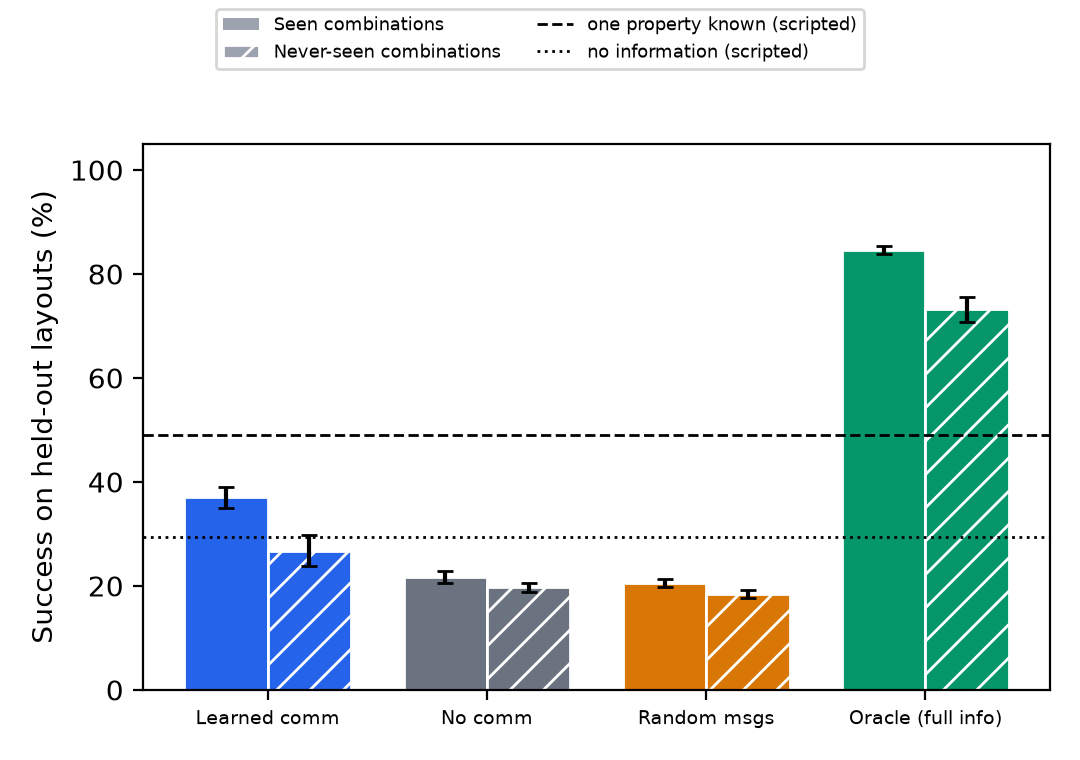
\includegraphics[width=\linewidth]{images/fig_v2_success.png}
\caption{Success on seen and never-seen color–shape combinations. Reference lines are scripted identification-and-navigation results, not learned baselines.}
\end{figure}

\textbf{Interventions and property-level behavior.} Whole-message
permutation tests whether the listener depends on the learned message
identities. The word-specific interventions localize sensitivity but do
not, by themselves, assign a property meaning to a word.

\begin{center}
\small
\resizebox{\columnwidth}{!}{%
\begin{tabular}{@{}
  >{\raggedright\arraybackslash}p{(\linewidth - 4\tabcolsep) * \real{0.3333}}
  >{\raggedright\arraybackslash}p{(\linewidth - 4\tabcolsep) * \real{0.3333}}
  >{\raggedright\arraybackslash}p{(\linewidth - 4\tabcolsep) * \real{0.3333}}@{}}
\toprule\noalign{}
\begin{minipage}[b]{\linewidth}\raggedright
Measure
\end{minipage} & \begin{minipage}[b]{\linewidth}\raggedright
Seen combinations
\end{minipage} & \begin{minipage}[b]{\linewidth}\raggedright
Never-seen combinations
\end{minipage} \\
\midrule\noalign{}



Intact − permuted & +22.3 pp (95\% CI +20.2 to +24.3) & +12.2 pp (95\%
CI +9.2 to +15.3) \\
Intact − word 1 permuted & +10.0 pp (95\% CI +8.4 to +11.5) & +5.5 pp
(95\% CI +4.0 to +7.1) \\
Intact − word 2 permuted & +10.2 pp (95\% CI +8.4 to +11.9) & +6.9 pp
(95\% CI +4.8 to +9.1) \\
Intact − silenced & +24.6 pp (95\% CI +22.2 to +27.0) & not run by the
pre-registered plan \\
Color correct among picks & 68.2\% (95\% CI 65.8--70.7) & 60.1\% (95\%
CI 57.2--63.1) \\
Shape correct among picks & 71.1\% (95\% CI 68.5--73.7) & 62.0\% (95\%
CI 58.6--65.2) \\
Wrong picks retaining color only & 38.4\% (95\% CI 34.9--42.1) & 36.8\%
(95\% CI 33.6--40.0) \\
Wrong picks retaining shape only & 44.0\% (95\% CI 40.0--48.0) & 39.9\%
(95\% CI 36.0--43.7) \\
Wrong picks retaining neither & 17.6\% (95\% CI 15.1--20.1) & 23.3\%
(95\% CI 21.7--25.0) \\

\bottomrule
\end{tabular}}
\end{center}

\textbf{Lexicon and structural metrics.} Figure 8 shows the median comm
seed's first-message symbol frequencies. The pooled seed-level measures
below describe whether word positions align with properties; they are
consistent with compositional organization when the patterns agree, but
they are not categorical proof of compositionality.

\begin{center}
\small
\resizebox{\columnwidth}{!}{%
\begin{tabular}{@{}ll@{}}
\toprule\noalign{}
Descriptive measure, seen combinations & Mean \\
\midrule\noalign{}



Word 1 MI with color & 1.31 bits \\
Word 1 MI with shape & 1.49 bits \\
Word 2 MI with color & 1.34 bits \\
Word 2 MI with shape & 1.49 bits \\
Topographic similarity & 0.24 \\
Positional disentanglement & 0.16 \\

\bottomrule
\end{tabular}}
\end{center}

\begin{figure}[tb]
\centering
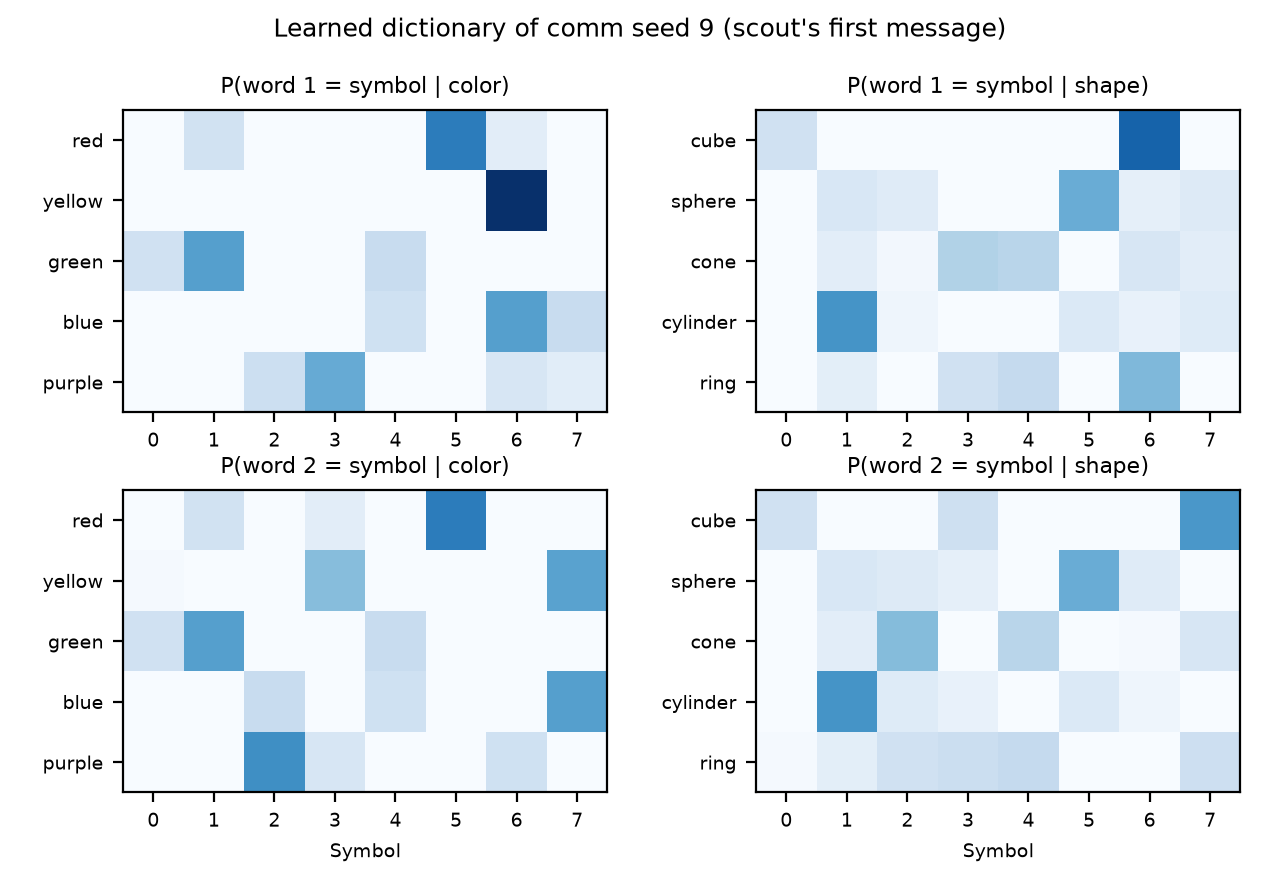
\includegraphics[width=\linewidth]{images/fig_v2_lexicon.png}
\caption{First-message symbol frequencies by target color and shape for the median comm seed. Any word–property alignment is descriptive and must be read together with the intervention and accuracy results.}
\end{figure}

\textbf{Unseen-support limitation.} The unseen target prior differs from
ordinary seen-square sampling. The five held-out pairs form a one-to-one
matching. A source-only exhaustive enumeration finds 80 equally likely
target--square states: 60 contain one held-out candidate and 20 contain
two. A strategy that knows only this support identifies the target
before navigation at 87.5\% in expectation; knowing either property plus
the matching identifies it at 100.0\%. This is a theoretical
identification calculation, not learned performance or navigation
success. Therefore H4 is exclusively a test of unseen success above the
fixed 50.0\% reference. It is not an unseen one-property ceiling and
does not establish transfer of both properties or compositionality.

\textbf{Interpretation.} Claim A was supported, but Claim B was not, so
Claim C was not reached. The experiment meets the seen-combination
communication criterion but not the pre-registered generalization
criterion. The unseen estimates and structural metrics remain
descriptive.

\section{Limitations}\label{limitations}

\begin{itemize}
\tightlist
\item
  \textbf{Toy scale:} one small world, one message per step, a
  single-step channel delay.
\item
  \textbf{Plug-in MI:} finite-sample bias affects the 200-episode
  estimates. No universal bias correction is assumed; MI remains
  descriptive and interventions carry the message-use claim.
\item
  \textbf{Privileged heuristic:} the scripted reference plans on the
  true map, so it is a headroom check and not a baseline.
\item
  \textbf{Tuning:} pilot tuning (configurations in the reproducibility
  section) used separate seeds and training layouts only. Any tuning
  choice still conditions the result on that configuration.
\item
  \textbf{v2 scale:} two properties with five values each, one fixed
  hold-out matching of five combinations, and one learning setup.
  Compositional generalization may behave differently with more
  properties, values, or hold-out structures.
\item
  \textbf{Method novelty and attribution:} cue-directed signalling is a
  task-specific adaptation of an existing information objective. The
  baseline ablation tests its value relative to unbiased IPPO in this
  task; it does not establish superiority to the full Eccles method or a
  new state of the art.
\item
  \textbf{Unequal extension budgets:} the vocal and compositional
  extensions use longer training than v1. Their absolute success rates
  are descriptive cross-task comparisons, not isolated tests of channel
  type or compositional difficulty.
\end{itemize}

\section{Reproducibility}\label{reproducibility}

The source, locked Python environment, per-seed tables, summaries,
preregistrations (\texttt{prereg-v1}, \texttt{prereg-v2}), deviations
and viewers are included. Train-only pilot selection used seeds
1000--1002 for v1 and 2000--2002 for v2. The table reports these small
selection studies, not benchmark evidence. The fixed decision tables
selected the biased v1 configuration and v2 rung 1 before benchmark
training.

\begin{center}
\small
\resizebox{\columnwidth}{!}{%
\begin{tabular}{@{}llll@{}}
\toprule\noalign{}
Train-only pilot & Comm & No comm & Oracle \\
\midrule\noalign{}



v1 pure IPPO & 21.8\% & 20.8\% & 87.2\% \\
v1 cue bias & 83.2\% & 20.8\% & 91.5\% \\
v2 rung 1 & 34.8\% & 19.5\% & 85.2\% \\
v2 rung 2 & 28.5\% & 19.5\% & 85.8\% \\

\bottomrule
\end{tabular}}
\end{center}

Deterministic CPU operations and seeded generators are enforced, and v1
weight/evaluation golden regressions remain intact. Bitwise agreement
across hardware or library versions is not assumed. The vocal arm was
declared exploratory before v1 pre-registration; the added
original-method ablation is post-hoc. Neither expands the original
confirmatory claims.

Static viewers illustrate exported trajectories. A separate
fresh-inference command loads the included representative final
checkpoints and produces new episode output for the live demo. Full
retraining uses the frozen commands; complete trained-run archives are
separate. The unseen-support calculation uses frozen source and
configuration without learned results. Later interpreter and stacking
proposals are not completed experiments in this report.

\textbf{AI assistance disclosure.} Claude and OpenAI ChatGPT/Codex
assisted with planning, implementation, checks and refinement of this
existing report. The November 9 request concerned course-requirement
auditing and submission preparation, including the exploratory ablation
and presentation materials. Details are in
\texttt{docs/AI\_ASSISTANCE.md}. The author remains responsible for the
text, implementation and interpretation, and supplies his own narration.

\textbf{References.}

\begin{itemize}
\tightlist
\item
  Jakob Foerster, Yannis Assael, Nando de Freitas, and Shimon Whiteson.
  \href{https://arxiv.org/abs/1605.06676}{\emph{Learning to Communicate
  with Deep Multi-Agent Reinforcement Learning}}. NeurIPS, 2016.
\item
  Angeliki Lazaridou, Alexander Peysakhovich, and Marco Baroni.
  \href{https://arxiv.org/abs/1612.07182}{\emph{Multi-Agent Cooperation
  and the Emergence of (Natural) Language}}. ICLR, 2017.
\item
  Ryan Lowe, Jakob Foerster, Y-Lan Boureau, Joelle Pineau, and Yann
  Dauphin.
  \href{https://ifaamas.org/Proceedings/aamas2019/pdfs/p693.pdf}{\emph{On
  the Pitfalls of Measuring Emergent Communication}}. AAMAS, pages
  693--701, 2019.
\item
  Tom Eccles, Yoram Bachrach, Guy Lever, Angeliki Lazaridou, and Thore
  Graepel. \href{https://arxiv.org/abs/1912.05676}{\emph{Biases for
  Emergent Communication in Multi-agent Reinforcement Learning}}.
  NeurIPS, 2019.
\item
  Christian Schroeder de Witt, Tarun Gupta, Denys Makoviichuk, Viktor
  Makoviychuk, Philip Torr, Mingfei Sun, and Shimon Whiteson.
  \href{https://arxiv.org/abs/2011.09533}{\emph{Is Independent Learning
  All You Need in the StarCraft Multi-Agent Challenge?}}.
  arXiv:2011.09533, 2020.
\item
  John Schulman, Filip Wolski, Prafulla Dhariwal, Alec Radford, and Oleg
  Klimov. \href{https://arxiv.org/abs/1707.06347}{\emph{Proximal Policy
  Optimization Algorithms}}. arXiv:1707.06347, 2017.
\item
  Rahma Chaabouni, Eugene Kharitonov, Diane Bouchacourt, Emmanuel
  Dupoux, and Marco Baroni.
  \href{https://aclanthology.org/2020.acl-main.407/}{\emph{Compositionality
  and Generalization in Emergent Languages}}. ACL, pages 4427--4442,
  2020.
\item
  Artemy Kolchinsky and Brendan D. Tracey.
  \href{https://www.mdpi.com/1099-4300/19/7/361}{\emph{Estimating
  Mixture Entropy with Pairwise Distances}}. Entropy 19(7):361, 2017;
  \href{https://www.mdpi.com/1099-4300/19/11/588}{correction}.
\end{itemize}
